\documentclass{beamer}
%
% Choose how your presentation looks.
%
% For more themes, color themes and font themes, see:
% http://deic.uab.es/~iblanes/beamer_gallery/index_by_theme.html
%
\mode<presentation>
{
  \usetheme{NYU}      % or try Darmstadt, Madrid, Warsaw, ...
  \usecolortheme{default} % or try albatross, beaver, crane, ...
  \usefonttheme{default}  % or try serif, structurebold, ...
  \setbeamertemplate{navigation symbols}{}
  \setbeamertemplate{caption}[numbered]
} 

\usepackage[english]{babel}
\usepackage[T1]{fontenc}
\usepackage[utf8x]{inputenc}
\usepackage{hyperref}
\usepackage{graphicx}
\title[ShortTitle]{EE2227: CONTROL SYSTEM}
\subtitle{Presentation 1 \\ GATE: 2017 ECE Q17 }\\
%\subtitle{GATE:2017 ECE Q19}
\author{KOIDALA SURYA PRAKASH}
\institute{EE18BTECH11026}
\date{\tomorrow}
%\titlegraphic{\hfill
\includegraphics[height=1.5cm]{nyu_shanghai}}

\begin{document}

\begin{frame}
  \titlepage
\end{frame}

\begin{frame}{Question}
  \Q. Consider the state space realization : \vspace{2mm}\\
 $$\left[\begin{array}{l}
\dot{x_{1}(t)} \\
\dot{x_{2}(t)}
\end{array}\right]=\left[\begin{array}{cc}
{0} & {0} \\
{0} & {-9}
\end{array}\right]\left[\begin{array}{l}
{x_{1}(t)} \\
{x_{2}(t)}
\end{array}\right]+\left[\begin{array}{c}
{0} \\
{45}
\end{array}\right] u(t)$$ \smallskip  \\
with the initial conditions $$\left[\begin{array}{l}
{x_{1}(0)} \\
{x_{2}(0)}
\end{array}\right]=\left[\begin{array}{l}
{0} \\
{0}
\end{array}\right] $$, where u(t) denotes unit step function  \vspace{2mm} \\
\textbf { The value of } \textbf{\lim _{t \rightarrow \infty}|\sqrt{x_{1}^{2}(t)+x_{2}^{2}(t)}|} \textbf { is ? }

\end{frame}


\begin{frame}{Theory}
\textbf{State Space Reprensentation} : \text{A state-space representation is a mathematical model of a physical}\\
\\system as a set of input, output and state variables related by first-order differential equations.
\\\textbf{For Linear systems : }
\\$$\dot{\mathbf{x}}(t)=A(t) \mathbf{x}(t)+B(t) \mathbf{u}(t)$$
\\ where $\dot{\mathbf{x}}(t):=\frac{\mathrm{d}}{\mathrm{d} t} \mathbf{x}(t)$
\\$$\mathscr{L}\{x(t)\}=X(s)$$
\\$$\mathscr{L}\{\dot{x(t)}\}=sX(s) - x(0)$$
%\\$$\mathscr{L}\\{dot{x(t)\}=X(s)$$
\end{frame}
 
\begin{frame}{Solution}
\left[\begin{array}{l}
\dot{{x_{1}(t)}} \\
\dot{{x_{2}(t)}}
\end{array}\right]=\left[\begin{array}{cc}
{0} & {0} \\
{0} & {-9}
\end{array}\right]\left[\begin{array}{l}
{x_{1}(t)} \\
{x_{2}(t)}
\end{array}\right]+\left[\begin{array}{c}
{0} \\
{45}
\end{array}\right] u(t) \vspace{5mm}\\
\text By applying Laplace transform on both sides, we get
$$
s X_{1}(s)-x_{1}(0)=0
$$
$X_{1}(s)=\frac{x_{1}(0)}{s}=0 \quad$     $\text \quad \because x_{1}(0)=0$
\\So, $\quad x_{1}(t)=0$\\
and $\quad s X_{2}(s)-x_{2}(0)=-9 X_{1}(s)+\frac{45}{s}$


\end{frame}

\begin{frame}{Solution}
$$
\begin{aligned}
\text { Required value } &=\lim _{t \rightarrow \infty}|\sqrt{x_{1}^{2}(t)+x_{2}^{2}(t)}| \\
&=\left|\lim _{t \rightarrow \infty} x_{2}(t)\right|
\end{aligned}
$$

$\lim _{t \rightarrow \infty} x_{2}(t)=\lim _{s \rightarrow 0} s X_{2}(s)=\frac{45}{9}=5$ \vspace{5mm}\\
$\mathrm{So}$
Required value $=|5|=5$
\end{frame}

\begin{frame}{Verification}
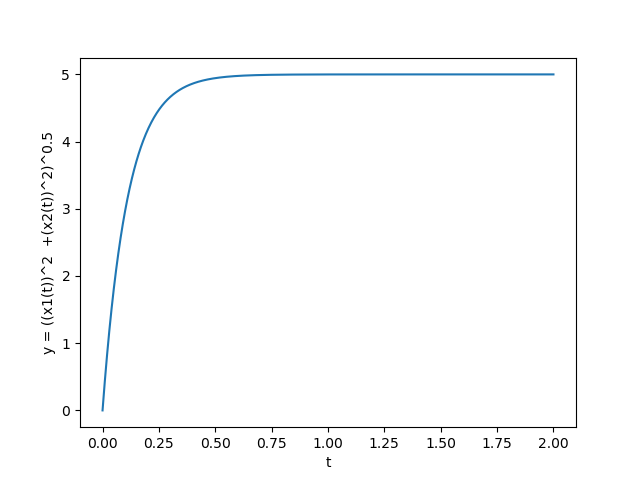
\includegraphics[scale=0.65]{gvv.png}

\end{frame}
\end{document}
